\chapter{Info Corso}
Esame progetto da sviluppare da soli, da fare in 3 settimane (esce un mese prima della data dell’esame), poi si discute all’orale con domande di teoria.\\
Errori di gestione della memoria causano insufficienza(memory leaks).

\chapter{C++}
\section{Introduzione}
Efficiente, molto performante in quanto di medio basso livello.
Deve poter dare al programmatore più stili di programmazione (procedurale/modulare/ObjectOriented/generica). Nasce dalla fusione di simula(Oggetti) e C.\\
Poche librerie già fornite, per mantenere le prestazioni buone, se voglio fare cose grosse devo cercarmele. Può essere che però le librerie siano platform based.
Dichiarare non alloca memoria, definire si.

\section{Compilazione}
\textcolor{dkgreen}{file.c}\\
\textcolor{red}{Preprocessore}(genere un testo con eventuali modifiche)\\
\textcolor{dkgreen}{unità di compilazione}\\
\textcolor{red}{Compilatore}(da fare per ogni file)\\
\textcolor{dkgreen}{codice.obj} (uno per ogni file)\\
\textcolor{red}{Linker}(unisce i vari file obj e le librerie)\\
\textcolor{dkgreen}{eseguibile}\\

Spesso Preprocessore e Compilatore sono uniti. Il file obj NON è portabile ne su altri sistemi  ne su altri compilatori. Possibilità di ricompilare solo i file sorgente modificati.
Il preprocessore effettua solo modifiche e sostituzioni testuali(STRINGHE), seguendo le direttive del codice sorgente(denotate da \#).

\section{Comandi Preprocessore}
\begin{itemize}
\item \#DEFINE permette di definire macro, in modo che se vengono trovate corrispondenze nel sorgente, il preprocessore gli sostituisce il valore della macro(SOLO PER STRINGHE). Si usano per i tag, stringhe senza valore che posso usare in combinazione con \#ifdef. NON SI USANO PER COSTANTI.
\item \#INCLUDE inserisce brutalmente il codice di un altro file, se uso le “” lo cerca nella cartella corrente, se uso le <> le cerca nelle cartelle di sistema.
\end{itemize}

\section{Compilatore}
Il compilatore esegue un'analisi sintattica del codice.\\
Il compilatore esegue un'analisi semantica del codice(controllo tipi, inizializzazione variabili\dots).\\
Il compilatore compila un file sorgente alla volta. Deve identificare quello che non è in quel file ma che sarà in altri file e vi inserise un segnaposto, in modo da poi sostituirla tramite il linker.\\
Infine crea il file binario con le microistruzioni e può ottimizzare il codice.

\section{Linker}
Il linker analizza tutti i file oggetto insieme e risolve i vari segnaposto, in modo da fondere correttamente il tutto. Aggiunge poi librerie e istruzioni particolari per ogni macchina.\\
Il linker elimina evenuali funzioni non usate scritte nel codice sorgente e poi compilato. Se qualcosa non è usato, viene rimosso.

\section{Riga di comando}
Per complilare:

\begin{tcolorbox}
g++ -c main.cpp -o main.obj 
\end{tcolorbox}

La parte -0 serve per rinominare il file di output\\
Per linkare:

\begin{tcolorbox}
g++ main.obj -o main.exe
\end{tcolorbox}

Per eseguire: 

\begin{tcolorbox}
./main.exe
\end{tcolorbox}

Per creare e eseguire direttamente l'eseguibile(se non ho altri files) uso:\\

\begin{tcolorbox}
g++ main.cpp -o main.exe
\end{tcolorbox}

Procedura per compilare più file e linkarli:\\

\begin{tcolorbox}
g++ -c main.cpp -o main.obj\\
g++ -c funct.cpp -o funct.obj\\
g++ main.obj funct.obj -o main.exe\\
\end{tcolorbox}

Se esegue questo comando, compilo tutti i cpp della directory e li linko:

\begin{tcolorbox}
g++ *.cpp -o main.exe
\end{tcolorbox}

Per passare alla versione senza assert e debug vari, aggiungo dopo g++ l'opzione -DNDEBUG\\
Le assert verificano dei parametri booleani, se non sono verificate, il programma si blocca. Se lo compilo con NDEBUG, si disattivano! Il concetto è che deve essere il chiamante a verificare che i dati passati siano sensati.

\section{Header File}
L'header file serve per rendere accessibili le funzioni e gli attributi di una classe all'esterno della stessa. Infatti i metodi per essere chiamati da un'altra classe, devono essere dichiarati in un header file e inclusi nella classe che li utilizza tramite la direttiva al preprocessore \verb|#INCLUDE| \\
Ciò permette al compilatore di "riconoscere" la firma dei metodi quando vengono chiamati, altrimenti verrebbe restituito un'errore.\\
E' buona pratica creare per ogni file diverso dal main, il file.h contenente le dichiarazioni delle funzioni ed il corrispondente file .cpp, dove devo ricordarmi la direttiva per il preprocessore \verb|#INCLUDE| \\

\begin{cpp}
#ifndef NOMEFILE_H
#define NOMEFILE_H
robachedefinisco
#endif
\end{cpp}

\section{Tipo}
Oltre ai soliti tipi come in java, esistono anche puntatoti e reference: non contengono dati, ma contengono una sorta di link indiretto per accedere al dato.\\
Per i tipi primitivi, esistonodelle keyword che permettono di cambiare le dimensioni dei dati(long, unsigned, short). Short e long posso essere usati direttamente al posto di int, non cambia nulla scrivere short int oppure short.\\
L'istruzione sizeof() ritorna la dimensione occupata dal dato, misurata in char(1 byte, 8 bit).

\section{Construtti base}
Le istruzioni if else sono come java, cosi come il ciclo for, while e do while, così come lo switch. Eccone alcuni esempi:

\begin{cpp}
for(int i=0; i<10,i++){
		
}

switch(var){
		case valore: istruzioni break;
		case valore: istruzioni break;
		case valore: istruzioni break;
		case valore: istruzioni break;
		default: istruzioni
	}
\end{cpp}

\section{Puntatori}
Sono un indirizzo di memoria che permettono l'accesso indiretto a un dato di un tipo definito:

\begin{cpp}
tipo *nomevariabile = 0; 
\end{cpp}

Se non viene inizializzato, punta ad una cella di memoria randomica! Molto pericoloso, BISOGNA SEMPRE ASSEGNARGLI 0.\\
Per ottenere l'indirizzo in memoria di una variabile, antepongo \& al nome della variabile e la posso così assegnare ad un puntatore.\\
Per dereferenziare un puntatore antepongo * al nome del puntatore e la assegno a una variabile.\\
Più puntatori possono puntare alla stessa area di memoria.\\
Sommando una cifra n ad un puntatore, lo sposto di n posizioni(del suo tipo) consecutive in memoria. Sottrarre due puntatori restituisce il numero di elementi(del tipo dei puntatori) tra i due indirizzi. La lunghezza dei puntatori è una quantità standard, a prescindere dalla dimensione del dato puntato.

\begin{cpp}
int i1 = 5;
double d1 = 1.45;

int *pi = &i1;
double *pd = &d1;

int datopuntato = *pi
\end{cpp}

\section{Array}
Gli array sono celle contigue in memoria. Non è niente altro che un puntatore alla prima cella in memoria. Se non inizializzati contengono dati casuali.

\begin{cpp}
int array1 [10];
\end{cpp}

\section{Reference}
Serve per assegnare un secondo nome ad una variabile. Si può assegnare solo un fase di instanziazione!\\
Simili ai puntatori, ma hanno una sintassi diversa: non vanno dereferenziati, ma si usano così come sono. Usati nel passaggio di variabili a funzioni.\\
Non possono puntare a NULL e non sono riassegnabili

\begin{cpp}
int target;
int &nomereference = target;
\end{cpp}

\section{Struct}
Struttura dati che contiene a sua volta diversi tipi di dati. Si accede ai campi con la notazione dot. E' simile ad una classe con variabili pubbliche.

\begin{cpp}
struct Punto {
	int x;
	int y;
};

Punto pt1;
pt1.x = 1;
pt1.y = 5;

//Se utilizzo puntatori, cambia la notazione

Punto *ppt = &pt1;
ppy -> y = 3;
\end{cpp}

Se creo due struct e faccio oggettostruct2=oggettostruct1 i dati vengono copiati da 1 in 2, rimanendo oggetti separati.\\
La dimensione in memoria di una struct è variabile, non sempre è la somma delle dimensione dei dati membro.

\section{Stringhe Primitive}
Array di caratteri terminati da un carattere speciale \verb|\0|\\
Sono compatibili con il C. Sono direttamente compatibili con il cout.\\

\begin{cpp}
char strc[10]="Buona"; 
char strl[]={'G','i','o','r','n','a','t','a','\0'}; 
\end{cpp}

Utili solo nel main quando prende degli argomenti da linea di comando(altrimenti uso le string contenute nella libreria string).

\begin{cpp}
int main(int argc, char *argv[])
{
// argc : numero di parametri passati al programma
// argv : array di puntatori a char (stringhe C) con i parametri
return 0;
}
\end{cpp}

argv è un array di puntatori a char, cioè un'array di stringhe primitive. All'indice 0 c'è il nome dell'eseguibile, dall'1 in poi vi sono gli argomenti.

\section{Typedef}
Typedef permette di creare dei nuovi tipi a partire dai dati di tipo base. Posso usare un typedef su un altro typedef in modo da modificare tutti i dati del tipo precedente.

\begin{cpp}
typedef unsigned long int tipopersonalizzato1;
tipopersonalizzato1 x = 123;
\end{cpp}

Utilizzo un typedef per i tipi dei miei attributi della classe, in modo da mascherare all'utente il tipo reale del mio attributo. Questo mi garantisce maggior sicurezza e mi permette di modificare il tipo in futuro in un solo punto del codice in caso di necessità. Oltre che all'attributo stesso, il tipo definito va usato nel suo getter e in generale ovunque sia utilizzata una variabile del tipo definito.

\section{Const}
Anteporre const ad una variabile in fase di dichiarazione e definizione la rende non modificabile. Posso anche rendere costante un reference, in modo che una variabile sia costante se accedo dal reference, ma modificabile se accedo da altro nome.

\begin{cpp}
const int *p;		//p e' un puntatore a intero const. Il dato non e' modificabile, il puntatore e' invece modificabile
int *const p;		//p e' un puntatore costante a un intero. Il dato e' modificabile ma il puntatore non puo' essere modificato.
const int *const p;		//tutto costante, non puo' essere modificato nulla.
\end{cpp}

Anteporre const al metodo indica che la variabile ritornata è costante. Se lo metto al termine della dichiarazione invece indico che il metodo non cambia lo stato della classe, quindi è chiamabile da variabili costanti.
Il const prima dei parametri del metodo invece, indica che essi non verranno modificati dal metodo.

\section{Cast}
Ho vari tipi di cast, a seconda del loro utilizzo. Il classico è quello statico, che permette di modificare il tipo della variabile. Il const cast permette di rimuovere a puntatori e reference l'immutabilità della variabile puntata. Il reinterpret serve per fare modifiche sui byte del dato(usato pochissimo)

\begin{cpp}
static_cast<tipodestinazione>(variabile);
const_cast<tipodestinazione>(variabile);
reinterpret_cast<tipodestinazione>(variabile);
\end{cpp}

\chapter{Funzioni}
NON FARE MAI return di puntatori o reference di variabili locali. Nei parametri posso usare un assegnamento con un valore di default. In caso la chiamata di funzione venga chiamata senza quel parametro, verrà utilizzato quello di default. Si parte a inserirli dal fondo:

\begin{cpp}
void f(char c=10, int v=90);
f(1, 29);
f(1); // esegue f(1,90)
f(); // esegue f(10,90)
\end{cpp}

Se antepongo la keyword inline prima del nome della funzione, essa evita il contex switch. Si usa per funzioni semplici semplici di pochissime righe.

\section{Passaggio di parametri}
\subsection{Passaggio per valore}
Quello che viene passato, viene inizalizzato dal chiamante.
All'atto della chiamata, viene creata una nuova variabile locale in memoria, creando copie dei dati. Le modifiche avvengono solo sulle variabili locali, alla fine della chiamata vengono eliminate.

\subsection{Passaggio per puntatore}
Quello che viene passato viene inizalizzato dal chiamante, nella chiamata a funzione si passa l'indirizzo della variabile.
La funzione riceve un puntatore, qualunque modifica sul puntatore dereferenziato, si ripercuote sulla variabile di partenza in modo permanente. Non occupo memoria extra e creo condivisione.

\subsection{Passaggio per reference}
Quello che viene passato, viene inizalizzato dal chiamante. Il chiamante passa la variabile come nel passagio per valore, ma la funzione riceve un reference. Questo crea condivisione, non una copia dei dati e quindi le modifiche sono definitive. E' come un pasaggio per puntatore, ma viene mascherata la sintassi di dereferenziazione.

\section{Extra}
Se voglio fare in modo che i dati putati da reference o puntatore non debbano essere modificati, allora devo chiamarre funzioni che garantiscano la constness dei parametri.\\
Per passare array devo per forza usare i puntatori. Ma se lo faccio non ho alcuna informazione sulla dimensione dell'array puntato, che rimane nel chiamante. Il trucco è passare anche un dato int che contenga la dimensione dell'array.\\
Se passo una struct che contiene puntatori e dati primitivi per valore, i dati vengono copiati, ma il puntatore punta alla stessa aera di memoria, quindi se modifico il dato puntato, essa si ripercuote. STARE MOLTO ATTENTI A PASSARE LE STRUCT, NON VI E' PROTEZIONE.\\

\chapter{Vita dei Dati}
Variabili locali nascono e muoiono in modo automatico nel loro scope. Sono visibili all'interno del loro scope(graffe). Se uso la keyword static, allora spravvivono alla fine della funzione e mantengono il valore, ma la visibilità rimane di scope. \\
Le variabili globali sono quelle dichiarate fuori dal main e dalle funzioni e dai namespaces. Sono leggibili da ogni punto del programma, create all'inizio dell'esecuzione del programma. Con la keyword extern nel file.h, una variabile può essere usata in tutti i file cpp che includono quell'header.\\
Le variabili dinamiche vengono create manualmente nella memoria RAM(HEAP) del sistema, su richiesta del programmatore. Non si distruggono da sole, devo usare delete per eliminare tutto quello che creo. Attenzione, se riassegno un puntatore che puntava a una variabile sull'heap, lo perdo e non posso più usarlo ne eliminarlo.

\chapter{Makefile}
Contiene le istruzioni "al contrario" della compilazione e del linking.\\
L'istruzione -I./include dice al compilatore di prendere gli header dalla cartella include.\\
Per lanciare il tutto basta lanciare il comando make e basta.\\
Se cambio un singolo file, il make ricompila solo quello modificato e linka il tutto.\\
File controllato dall'indentazione, fare attenzione!!

\begin{cpp}
main.exe: Point.o Rectangle.o main.o
	g++ Point.o Rectangle.o main.o -o main.exe

main.o: main.cpp
	g++ -I./include -c main.cpp

Point.o: ./src/Point.cpp
	g++ -I./include -c ./src/Point.cpp

Rectangle.o: ./src/Rectangle.cpp
	g++ -I./include -c ./src/Rectangle.cpp

.PHONY: clean
clean:
	rm -rf *.o main.exe
\end{cpp}

\chapter{Debuggigng}
\section{GBD}
Debugger logico da riga di comando

\section{Valgrind}
Programma che permette di verificare la presenza di memory leak e di errori in lettura/scrittura della memoria(Dinamica, non Statica).\\
Lo si invoca con \textit{valgrind nomeprogramma.exe}
In compilazione, durante le fasi di debug, è utile utilizzare:

\begin{tcolorbox}
g++ -g nomesorgente.cpp -o nomeprogramma.exe
\end{tcolorbox}

Questo permette di mostrare su Valgrind la riga di codice che genera errore.
Valgrind segnala i leak come memoria non deallocata oppure persa. Eventuale memoria "Still Reachable" non costituisce un problema!

\chapter{Classi}
Sono formati da classe.cpp e classe.h dove sono inserite solo le dichiarazioni di variabili e metodi. Le variabili all'interno delle classe hanno una convenzione: mettere il primo carattere \verb|_|\\
Tutto quello che è in una classe è privato di default, per rendere pubblico, uso la keyword public:\\
Tutto quello scritto sotto di essa è pubblico. Concetto di sezione, a differenza di java.
Nel file claasse.cpp devo usare in namespace per definire i metodi della classe stessa.

\section{Costruttori}
La prima cosa pubblica è il costruttore di default, fondamentale e obbligatorio. Ha il nome della classe e non prende parametri.
E' quello chiamato di default, e l'unico che può essere chiamato se alloco un'array di variabili. Per chiamarlo devo solo creare la variabile, il costruttore standard si chiama da solo.
Per creare un dato di tipo classe uso:

\begin{cpp}
nomeclasse novevariabile() : variabile=valore, variabile2=valore2;
nomeclasse nomevariabie(parametri) : variabile=valore, variabile2=parametro;
\end{cpp}

ATTENZIONE, se il costruttore prende un solo parametro, devoanteporre explicit nella dichiarazione del file .h \\
Il secondo costruttore obbligatorio è il copy constructor, che crea una copia del dato passato. Grazie ad esso, posso passare dei dati di tipo classe "per valore", in automatico si crea la copia del dato, vengono utilizzati e poi distrutti. Se invece passo tramite reference o puntatori, non si genera un nuovo dato e c'è condivisione di dati.

\begin{cpp}
nomeclasse(const nomeclasse &other);
\end{cpp}

I costruttori non si possono chiamare a vicenda. Nel costruttore è buona norma inizializzare le variabili e i dati tramite la initialization list. Questo permette di eseguire l'inizializzazione prima ancora che il costruttore venga effettivamente chiamato. Ciò permette di mantenere la massima coerenza nel caso in cui il costruttore fallisse.

\section{Distruttore}
Insieme al costruttore, devo creare il distruttore, che viene chiamato automaticamente alla terminazione dello scope della variabile. NON viene chiamato in automatico se alloco una variabile con il new.

\section{Ridefinizione operatori}
Posso ridefinire addirittura gli operatori, per fargli fare cose a piacere. Buona norma è ridefinire l'operatore di assegnamento = , il << per la stampa dell'oggetto e il [] per accedere ad un indice se è contenuto un'array.

\begin{cpp}
dbuffer &operator=(const dbuffer &other);
int &operator[](unsigned int index);
const int &operator[](unsigned int index) const;
std::ostream &operator<<(std::ostream &os, const dbuffer & db);
\end{cpp}

\section{Getter e Setter}
Non è buona norma usare getter e setter per ogni variabile come java, ma ritorno il reference alla variabile, in modo che funga per entrambi gli scopi. ATTENZIONE! Si crea sempre anche la versione con il const prima e dopo la dichiarazione, in modo che funzionino sia se vengono chiamati da dati variabili sia se vengono chiamati da dati const. Questo vale per qualunque cosa che potrebbe dare problemi se lavoro con variabili const.

\begin{cpp}
int &dbuffer::value(unsigned int index){
	assert(index < _size);
	return _buffer[index];
}

const int &dbuffer::value(unsigned int index) const{
	assert(index < _size);
	return _buffer[index];
}
\end{cpp}

\section{Metodi Fondamentali}
\begin{itemize}
\item COSTRUTTORE
\item DISTRUTTORE
\item COPY-COSTRUCTOR
\item ASSEGNAMENTO
\end{itemize}

\section{Gestione Errori}
Nel caso in cui una funzione lanciasse un errore ed esso non venisse gestito tramite un try catch, la funzione sarebbe immediatamente terminata e l'errore propagato al chiamante. Questo meccanismo può essere sfruttato direttamene dai costruttori: se una new fallisce, il costruttore termina immediatamente e propaga l'errore al chiamante. Non vi sono ovviamente leak di memoria, in quanto la new è fallita.\\
Si è soliti creare 2 metodi di creazione e accesso, in modo che sia l'utente a scegliere se utilizzare quello con o senza eccezioni.
Quando faccio il catch di un errore, non mi devo limitare a stampare a schermo il messaggio dell'errore, ma devo ripristinare(revovery) uno stato il più coerente possibile. Posso poi propagare ulteriormente l'errore al chiamante, in modo da informarlo dell'errore avvenuto.

\section{Ridefinizione operatori}
Possiamo ridefinire qualunque operatore nelle classi che definiamo. Lo faccio per definire comportamenti particolari deglio operatori nelle classi.\\
Possono essere operatori binari(+, -, *, =, /, =, \dots) oppure unari(++,!, --, +=, -=, \%, \dots).\\
Gli operatori sono fortemente legati al dato a sinistra, quindi solitamente non sono simmetrici.\\
Gli operatori di classe unari non possono ricevere parametri, quelli binari hanno un solo parametro. Se l'operatore è invece globale, hanno rispettivamente 1 e 2 parametri.\\
Gli operatori si possono solo ridefinire, mai creare.
Possono essere ridefiniti internamente o esternamente alla classe, dipende dall'operatore.\\
Esistono anche operatori di conversioni(sempre membri della classe).
Ecco un esempio:

\begin{cpp}
#include <iostream>

class complesso{
	double _real;
	double _imm;

public:
	//costruttore di default
	complesso();
	//costruttore con parametri
	complesso(double real, double imm);
	//distruttore
	~complesso();
	//copy constructor
	complesso(const complesso &other);
	//operatore di asseganemto
	complesso& operator=(const complesso &other);
	//ridefinisco * per accedere alla parte reale. Verisione lettura e scrittura.
	double &operator *();
	//versione solo lettura
	const double &operator *() const;
	//ridefinisco ! per accedere alla parte immaginaria. Verisione lettura e scrittura. GLOBALE( solo per esempio didattico), quindi due parametri
	double &operator !(complesso &c);
	//versione solo lettura. Non va cosnt alla fine perche' non e' una funzione membro, e' solo friend
	const double &operator !(const complesso &c);
	//Operatore prodotta tra numeri complessi
	complesso operator-(const complesso &dx) const;
	//prodotti tra numeri immaginari
	complesso operator*(const complesso &dx) const;
	//modulo del numero immaginario
	double operator+()const;
	//somma tra double e complesso
	complesso operator+(double dx)const;
	//essendo un'operazione che cambia l'oggetto stesso, deve tornare il membro di sx
	complesso &operator+=(const complesso &dx);
	//friend permette di accedere ai dati privati della classe
	friend std::ostream& operator<<(std::ostream& os, const complesso &c);
	//permette il cast automatico a intero
	operator int() const;

};

//somma tra due numeri immaginari
complesso operator+(const complesso &sx, const complesso &dx);
//non serve friend perche' non usa dati della classe in modo diretto
//sottrazione con autop assegnamento
complesso &operator-=(complesso &sx, const complesso &dx);
//operatore autoincremento prefisso
complesso &operator++(complesso &sx);
//operatore autoincremento postfisso(ritorna il vecchio valore dopo l'incremento). 
//Il parametri int e' farlocco, serve solo a differenziare la signature della funzione postfisso da una prefissa
complesso operator++(complesso &sx, int);
/*
Operatore rapporto scalare/complesso
Se sx = 1+i0 si ha il reciproco del numero complesso 
E' un operatore binario
*/
complesso operator/(const complesso &sx, const complesso &dx);
//Operatore coniugato di un numero complesso
//E' un operatore unario
complesso operator-(const complesso &c);
//Operatore di somma tra uno scalare e un numero complesso
complesso operator+(double sx,const complesso &dx);

\end{cpp}

\section{Classe Templata}
Una classe templata è un prototipo di classe in cui non è specificato il tipo di dato su cui si lavora. Si premette al nome della classe \textit{template <typename T>}\\
Tutte le operazioni devono essere indipendenti e funzionanti per qualunque tipo di dato venga utilizzato. Non si fa direttamente riferimento al tipo, ma ad un placeholder(solitamente si usa T) che lo sostituisce(sia nelle variabili sia nelle funzioni).\\
N.B. non posso più dividere le classi in cpp e h, devo mettere tutto nel fine h.\\
Se le funzioni e i metodi non sono della classe, devo premette al nome della funzione \textit{template <typename T>}\\
Non posso più utilizzare i tipi definiti con i typedef in modo diretto, ma devo scrivere: \textit{typename nomeclassetemplate<T>::tipodefinitonellatypedef}

\section{Funtori}
Sostituiscono gli operatori e ne incapsulano la logica. Vengono definiti dal chiamante quando i tipi di dato che si vogliono utilizzare non implementano direttamente l'operatore voluto. La sintassi è:

\begin{cpp}
struct compare_int{
	bool operator()(int a, int b)const{
		return a<b;
	}
};
\end{cpp}

Il chiamante istanzierà un oggetto di tipo funtore e lo passerà alla funzione che esegue l'operazione voluta insieme ai dati.\\
Si possono utilizzare funzioni globali al posto dei funtori, ma sono scomode e non hanno la possibilità di mantenere uno stato

\section{Iteratori}
Sono oggetti che servono per esplorare i dati delle classi container. La sorgente dei dati è la classe container stessa, gli iteratori offrono all'esterno un'interfaccua standard di accesso ai dati della classe. Creano quindi un layer tra l'accesso ai dati e l'effettiva struttura di memorizzazione utilizzata.\\
L'iteratore è una classe che viene definita all'interno della classe container stessa che deve iterare. La struttura della classe iterator è predefinita e ha uno scheletro fisso a seconda del tipo di iteratore che si vuole implementare.\\
I metodi che devono essere implementati, dipendono direttamente dalla struttura della classe(posso eseguire accessi randomici con le parentesi [] oppure devo andare in ordine?)\\

\begin{figure}[H]
\centering
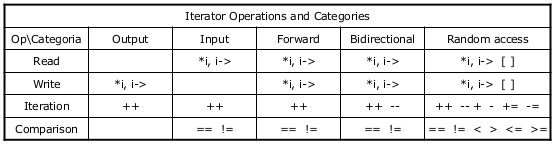
\includegraphics[scale=0.7]{Tab_iteratori}
\caption{Metodi degli iteratori}
\end{figure}

Vi deve sempre essere la versione costante corrispondente dell'iteratore(\verb|const_iterator|). Se non si vuole offrire possibilià di modifica dei dati, si definisce solo il \verb|const_iterator|\\
L'iteratore deve avere sempre due metodi principali, begin e end. Il primo se chiamato porta l'iteratore a puntare al primo elemento della classe. Possiamo spostarlo per puntare ai dati successivi. Il secondo metodo invece restituisce un iteratore che punta alla casella di memoria successiva all'ultimo dato.\\
Gli iteratori si creano sempre in coppia, uno punta all'inizio e uno alla fine. Quello che punta alla fine serve solo per capire se ho finito gli elementi, non mi serve per accedere ai dati o altro.\\
Ecco un esempio di utilizzo:

\begin{cpp}
//oggetto container a caso, fingiamo sia pieno
std::vector<int> v;

//creo i due iteratori. Non sono ancora legati a v
std::vector<int>::iterator it, ite;

//ciclo su tutti gli elementi. Il begin e l'end legano l'iteratore all'oggetto v
//Gli operatori sono stati ridefiniti nella classe iterator contenuta in vector
for (it = v.begin(), ite = v.end(); it != ite; it++){
	std::cout << *it << std::endl;
}
\end{cpp}

\chapter{Ereditarietà}
\section{Introduzione}
L'ereditarietà permette di acquisire caratteristiche da una classe esistente. Per esempio le forme geometriche hanno attributi comuni, che possono essere ereditati da un'entità superiore.\\
Per ereditare informazione da una classe, si scrive dopo il nome della classe derivata : public classedacuiereditare\\

\begin{cpp}
class people{
//...
};
class student : public people {
//...
};
\end{cpp}

In questo modo tutte le sezioni della classe padre, mantengono le caratteristiche. La classe derivata non ha accesso alla parte privata della classe padre, ma solo alla parte pubblica. Ha invece accesso a eventuali sezioni protette nei metodi della classe, ma dall'esterno potrò accedere comunque solo ai metodi ed ai dati public.\\

ATTENZIONE se ridefinisco una funzione con lo stesso nome della funzione della classe padre, anche se ha firma diversa, tutti i metodi con lo stesso nome della classe padre vengono automaticamente nascosti. Per richiamarli, devo usare una nomenclatura particolare.\\
\textit{oggettoderivato.classepadre::funzionepadre(parametri);}\\

\section{Costruttori}
Di default, sono chiamati i costruttori di default della classe padre e dei membri. Se voglio modificare il costruttore chiamato, devo listarli nella initialization list.\\
Un costruttore di una classe derivata deve per prima cosa chiamare il costruttore della classe padre per crearla. Si procede in cascata.  Dopo il costruttore della classe padre, sono chiamati i costruttori dati membro. Solo alla fine è chiamato il costruttore della classe derivata.

\begin{cpp}
class Derived : public Padre {
	Member m;
public:
	Derived(int) {} //costruttore default di Padre
	Derived(int,int) : Padre(123), m(0) {} //costruttore che chiama il costruttore della Padre(int) e m(int)
};
\end{cpp}

\section{Distruttori}
I distruttori sono chiamati automaticamente in ordine inverso rispetto ai costruttori(classe derivata, dati membro e classe padre). Non ho bisogno di alcuna sintassi particolare per la chiamata.

\section{CopyConstructor}
Se non implementato nella classe derivata(uso quello del compilatore che copia membro a membro), allora chiama il cc della classe padre e chiama i cc dei dati membro della derivata.\\
Se lo implemento io, devo fare io la chiamata a tutti i cc nella initialization list(prima della classe padre e poi dei dati membro).

\begin{cpp}
Derived(const Derived& other) : Padre(other), m(other.m) {...}
\end{cpp}

\section{Operatore di Assegnamneto}
Uguale al COPYCONSTRUCTOR, se lo implemento devo chiamare all'interno del corpo il copy constructor della classe padre usando il namespace.

\begin{cpp}
Derived &operator=(const Derived& other) {
	if (this != &other) {
		Padre::operator=(other);
		m=other.m;
	}
	return *this;
}
\end{cpp}

\section{UpCasting}
Upcasting significa passare da un classe derivata alla classe padre. Si può fare solo tramite puntatore o reference. Mi serve per la chiamata ai metodi base, oppure voglio creare metodi che usano oggetti della classe padre.\\
L'oggetto originario continua a esistere, vengono solo nascoste le specificità.

\begin{cpp}
Padre &b=derivata;
Padre *b=&derivata;
\end{cpp}

\section{DownCasting}
Attenzione, solitamente non è sicuro! Lo posso fare solo su classi polimorfe. Si fa su puntatori o reference tramite il dynamic cast\\

\begin{tcolorbox}
VarDerivata = dynamic\verb|_|cast<TipoDerivata>(VarPadre)
\end{tcolorbox}

\section{Polimorfismo}
La keyword virtual messa prima di un metodo, permette di utilizzare il metodo in modo polimorfo. Se viene ereditato, esso rimane polimorfo.
In questo modo, il metodo diventa polimorfo e, se chiamo un metodo virtual del padre su un oggetto derivato upcastato al padre, viene chiamato il metodo del figlio.\\
Se definisco virtual il distruttore, posso fare questo per esempio(altrimenti, si chiamerebbe solo il distruttore di Instrument e perderei il distruttore di Harp):

\begin{cpp}
int main(void) {
	Instrument *i = new Harp;
	//...
	delete i;
}
\end{cpp}

\subsection{Classi Astratte/Interfacce}
Se definisco un metodo virtuale puro, scrivendo =0 dopo il metodo, esso renderà la classe astratta, quindi non istanziabile. 

\begin{cpp}
virtual valoreritorno nomemetodo(params)=0;
\end{cpp}

Solo le classi derivate che fanno override del metodo virtuale puro possono essere istanziati.\\
Per creare un'interfaccia, tutti i metodi saranno virtuali puri.

\chapter{Doxygen}
Strumento che rende possibile la creazione di documentazione a partire dai commenti contenuti nei files.
Si utilizza la sintassi seguente:
All'inizio di ogni file, dopo le varie include, si scrive

\begin{cpp}
/**
@file nomefile
@brief Descrizione del contenuto(ES: dichiarazione della classe dbuffer)
**/

/**
@brief Cosa e' la classe in una riga

Descrizione dettagliata della classe
**/
\end{cpp}

A fianco ai dati membro della classe, si usa la sintassi \verb|\\\< descrizione| per dire cosa rappresentano quei dati
\newpage
Per documentare i metodi invece si scrive prima del metodo stesso:

\begin{cpp}
/**
	@brief Descrizione del metodo 
	Eventuale descrizione aggiuntuva del metodo
	@pre descrizione di eventuali condizioni da verificare(assert)
	@param nomeparametro descrizione parametro
	@param nomeparametro2 descrizione parametro2
	@return descrizione di cosa viene ritornato
	@throw eccezionelanciata descrizione di quando viene lanciata l'eccezione
*/
\end{cpp}

Ovviamente non sono tutti necessari, scelgo io quali inserire

\chapter{Standard 11}
Inserimento di nuovi tipi(long long è un intero a 64 bit, nullptr è un puntatore a null, \dots) \\
Introduce la keyword auto in fase di inizializzazione, che assegna automaticamente il tipo a una variabile o a una funzione.
Introduce decltype, una funzione che estrae il tipo di una variabile precedentemente inizializzata(anche su variabili auto).\\ 
Introduzione delle funzioni lambda.
Possibilità di chiamare i costruttori a vicenda.\\
Possibilità di creare array statici sullo stack.\\
Introduzioni di nuove funzioni per il tempo.\\

\chapter{Multithreading}
Si ottiene utilizzando OpenMP(API integrata nei complilatori) e consiste in 3 elementi:

\begin{itemize}
\item Direttiva al compilatore (indica al compilatore le regioni da parallelizzare)
\item Funzioni a runtime
\item Variabili di ambiente
\end{itemize}

La compilazione deve essere eseguita con il parametro -fopenmp \\
Concetto di fork e join. Il programma inizia con un solo thread, quando trova una regione OMP con le direttive, vengono generati dei thread secondari che vivono nella regione OMP e muoiono all'uscita, sincronizzandosi con la master.\\
Tutte le direttive di OpenMP iniziano con

\begin{tcolorbox}
\verb|#pragma omp parallel [clauses]|
\end{tcolorbox}

E' necessario includere <omp.h> per usare una serie di funzioni per avere accesso a informazioni su numero di thread e id del thread in cui ci troviamo.\\
Le variabile esterne alla regione OMP sono condivise tra i vari thread di default, cosa che può causare rece condition. Posso forzare a creare una copia privata, prevenendo così la race condition(l'esistenza delle variabili condivise permane, ma non vengono utilizzate)\\
Posso creare una omp sections che contiene diverse omp section, in modo che siano eseguite in parallelo.

\section{Chunk}
Se modifico la direttiva in 

\begin{tcolorbox}
\verb|#pragma omp parallel SCHEDULE(DYNAMIC, chunk_size)|
\end{tcolorbox}

Questo crea dei chunk di dati in modo dinamico  che vengono assegnati ai thread, il primo che termina ne riceve altri, in modo da gestire in modo automatico il load balancing e permettere la terminazione del compito in modo contemporaneo.

\section{Sincronizzazione}
OpenMP mette a disposizioni diverse direttive per gestire le
sincronizzazioni tra thread:

\begin{itemize}
\item OMP MASTER = Solo il thread master può eseguire il blocco di codice seguente. Gli altri thread non attendono il master thread.
\item OMP CRITICAL = Solo un thread può eseguire il blocco di codice seguente. Gli altri thread che raggiungono questo blocco rimangono in attesa. Quando il precedente thread finisce, eseguono a loro volta il codice.
\item OMP BARRIER = Tutti i thread devono raggiungere la barriera prima di proseguire. Nel frattempo i thread rimangono in attesa dei ritardatari.
\end{itemize}

La direttiva reduction permette di evitare molteplici modifiche a una variabile condivisa da parte di più thread, come in questo caso

\begin{cpp}
sum = 0;
#pragma omp parallel for shared(sum, a) reduction(+: sum)
for (int i=0; i<9; ++i){
	sum += a[i]
}
\end{cpp}

\chapter{Librerie}
Aumentano la versatilità del codice sorgente, è un'alternativa alla creazione e inclusione di header file. E' una collezione di funzioni usata per sviluppare applicazioni. E' più rapida dei files header, la loro condivisione è limitatata alla conoscenza della signature delle funzioni.\\
Permette riutilizzo, condivisione e organizzazione del codice.
Esistono due tipi di librerie, statiche e dinamiche. 

\section{Statiche}
In fase di linking, viene verificato quali funzioni sono usate nel codice e non sono presenti nel sorgente. Il linker cerca nelle librerie e le linka, inserendole fisicamente nel codice.\\
Per il linking, devo usare l'opzione -l per specificare il nome della libreria, -L percorsodellalibreria per indicare dove si trova(se è nella dir corrente metto L.) e -I percorso header della libreria(se sono nella stessa dir non metto la I).\\
Per generare una libreria, uso:

\begin{tcolorbox}
g++ -c nomefiles.cpp 
ar rcs libnomelib.a nomefiles.o
\end{tcolorbox}

Per compilare il sorgente invece uso in entrambi i casi:
\begin{tcolorbox}
g++ -o main.exe main.cpp -L percorso -l nome(senza lib davanti e senza estensione) -I percorsoheaderfiles
\end{tcolorbox}

Vengono estratti solo i moduli necessari alla compilazione, ma ciascun programma contiene una copia di quel codice, quindi i requisiti di memoria si moltiplicano

DINAMICHE
Sono anche dette librerie condivise: non viene vopiato il codice dalla libreria, vengono eseguite a runtime le porzioni di codice direttamente dalla libreira. Rimangono codici separati. Il linker non copia, semplicemente verifica che le funzioni usate siano disponibili.\\
Quando si esegue il programma, il sistema operativo la cerca in un modo peculiare(windows le carica all'avvio del programma, unix all'invocazione della funzione).\\
Hanno il vantaggio di essere caricate solo se usate e di potr modificare la libreria senza ricompilare il programma
Per crearle uso:

\begin{cpp}
g++ -fPIC -c files.cpp
g++ -shared -o libnomelibreria.so nomefiles.o
\end{cpp}

Per compilare il sorgente invece uso in entrambi i casi:
\begin{tcolorbox}
g++ -o main.exe main.cpp -L percorso -l nome(senza lib davanti e senza estensione) -I percorsoheaderfiles
\end{tcolorbox}

\chapter{QT}
E' uan libreria open source cross platform. Supporta diversi compilatori, tra cui gcc. QT implementa e migliora la capacità di scrivere codice astraendo parti che eravamo costretti a gestire in c++\\
Concetto di condivisione implicita. Tutto quello gestito da QT è gestito tramite copie per reference. Viene creata una copia shallow, quindi copiato solo il puntatore; se avvengono modifiche su questi dati, allora si crea una copia del dato e modificata la copia fatta, in modo da non influire su altre classi che puntano il dato. Inoltre vi è per ogni oggetto un referencecount che conta appunto quanti reference/puntatori stanno puntando l'oggetto. Se arriva a 0, lo posso eliminare.\\
Tutti i main iniziano e finiscono con queste due istruzioni:

\begin{tcolorbox}
QApplication app(argc, argv);\\
return app.exec();
\end{tcolorbox}

Qapplication è il gestore degli eventi del SO, mentre l'istruzione exec() è il while infinito che gestisce gli eventi.

\section{Modello a oggetti}
Alcuni attributi sono visti come proprietà definite all'interno degli oggetti. Posso accedervi sia in lettura che scrittura con le funzioni:\\

\begin{tcolorbox}
QObject::property()\\
QObject::setProperty()
\end{tcolorbox}

Posso aggiungere le proprietà in modo dinamico, infatti setProperty chiamata su una istanza di un oggetto, crea la proprietà se essa non è già presente.\\

La gestione degli eventi avviene tramite oggetti della classe QEvent. Possono essere gestidi da qualunque istanza della classe QObject, da cui derivano tutti i widget. Posso eseguire l'override delle funzioni per gestire gli eventi, in modo da modellare la gestione a mio piacimento.\\
Un widget è un elemento visuale della interfaccia utente(bottone, barra, menu, \dots). Sono componibili e si possono contenere l'un l'altro.

\section{Compilazione}
Creo un file .cpp con all'interno il codice. Il primo comando crea il progetto, con estensione .pro, il secondo crea il makefile e il terzo avvia la compilazione che produce l'eseguibile

\begin{tcolorbox}
qmake -project -o nomefile.pro\\
qmake nomefile.pro\\
make
\end{tcolorbox}

\section{Widget}
Hanno tutti il metodo show, che serve per renderli visibili. Tutti gli oggetti grafici sono oggetti che "vivono" in un oggetto contenitore, che non è altro che un puntatore ad un widget. Attraverso questi puntatori ho una gerarchia che rappresenta chi contiene cosa. Questo permette al gestore di eventi di capire fino a dove inviare l'evento. Il codice dei pulsanti e i vari widget sono contenuti nella ui viene generato automaticamente.

\paragraph{Label}
Qlabel è un widget utilizzato per visualizzare contenuti senza interazione con l'utente. E' come una cella nella quale viene inserito il contenuto. Posso inserire testo(\textit{QString::setText()}), immagini (\textit{QPixmap::setPixmap()}), video.\\
Di default il contenuto inserito è allineato a destra, ma posso settarlo tramite le funzioni \textit{setAlignment() e setIndent()}.\\

\paragraph{Button}
Crea un bottone con una scritta. Può essere associato ad eventi, in modo da gestire la pressione su di esso. Per esempio:\\

\begin{tcolorbox}
QPushButton *button = new QPushButton("Quit");\\
QObject::connect(button, SIGNAL(clicked()), \&app, SLOT(quit()));\\
button->show();
\end{tcolorbox}

\paragraph{Widget personalizzati}
Sono definiti come normali classi C++, con la particolarità di estendere tutti la classe QWidget e avere primo dato \verb|Q_OBJECT|\\
Nel costruttore viene sempre chiamato nell initialization list il costruttore della classe padre con paramentro *parent, che è di default 0. Come descritto successivamente, posso definire nuovi slot personalizzabili per il widget creato

\section{Layout e finestre}
Un layout(manager) è un oggetto che imposta la dimensione e la posizione dei widget che risiedono al suo interno. Posizione e dimensione dei widget è automaticamente adattata in base alle dimensioni dei widget, tuttavia è possibile specificare manualmente tale informazione. Esistono tre diversi layout manager:\\

\begin{itemize}
\item QHBoxLayout posiziona i widget orizzontalmente da sinistra verso destra
\item QVBoxLayout posiziona i widget verticalmente dall’alto verso il basso
\item QGridLayout posiziona i widget all’interno di una griglia
\end{itemize}

Il layout è solitamente inserito in una finestra, che contiene uno o più layout. Layout e finestra si creano così:

\begin{tcolorbox}
	QWidget *window = new QWidget;\\
	QVBoxLayout *myLayout = new QVBoxLayout;\\
	myLayout->addWidget(widget1);\\
    myLayout->addWidget(widget2);\\
	window->setWindowTitle("Enter Your Age");\\
	window->setLayout(myLayout);\\
	window->show();
\end{tcolorbox}

\section{Segnali e slot}
QPushButton è un esempio di widget che permette interazione con l'utente, lanciando funzioni di altri widget/classi.

\begin{tcolorbox}
QPushButton *button = new QPushButton("Quit");\\
QObject::connect(button, SIGNAL(clicked()), \&app, SLOT(quit()));
\end{tcolorbox}

Il segnale clicked lanciato dal bottone è catturato da \&app e viene lanciata la quit dell'oggetto app. In generale avremo:\\

\begin{tcolorbox}
QObject::connect(sender, SIGNAL(signal), receiver, SLOT(slot));
\end{tcolorbox}

sender e receiver sono puntatori a QObjects, mentre signal e slot sono signature di funzioni senza i nomi dei parametri. SIGNAL() e SLOT() sono invece delle macro che convertono gli argomenti in stringhe.\\

Un segnale viene emesso quando si verifica una particolare interazione.
Uno slot è una funzione chiamata in risposta a un particolare segnale.\\
I widget forniscono molti slot predefiniti, ma è possibile aggiungere i propri slot in modo da poter gestire i segnali a cui si è interessati. Per farlo, creo nel file.h una sezione \textit{private slots:} e li inserisco la firma dei miei metodi SLOT. Nel file .cpp li implemento semplicemente.\\
La signature di un segnale deve coincidere con la signature dello slot ricevente. Posso combinare le connsessioni in diversi modi: un segnale a + slot, più segnali a uno slot, un segnale a un segnale.\\
IL gestore principale gestisce gli eventi del SO e li spedisce agli oggetti grafici, che a loro volta gestiscono gli eventi inviati.
I segnali invece sono messaggi secondari, più di alto livello, che si inviano gli elementi grafici tra di loro e si gestiscono con sistema signal e slot.\\
Eventi e segnali/slot sono due meccanismi paralleli in grado di ottemperare agli stessi scopi. Un evento viene generato da un'entità esterna ed è consegnato attraverso il ciclo degli eventi in QApplication.\\
Segnali/slot sono utilizzati per la comunicazione tra gli oggetti. I segnali sono utili quando si utilizza un widget, mentre gli eventi sono utili quando si implementa un widget. Un esempio di evento è la pressione di un tasto o il click del mouse. 
Solitamente l'evento è un input dall'esterno non associato ad un particolare elemento nella ui. Serve per modificare il comportamento di default del widget all'avverarsi di un evento.\\
Le classi che implemento implementano dei metodi virtuali che corrispondono agli eventi. Se li voglio gestire, basta farne l'override nel file .h e poi implementarlo nel cpp.\\

\section{Filtering e coda di eventi}
A volte un oggetto deve osservare e possibilmente intercettare gli
eventi che vengono consegnati a un altro oggetto: la funzione

\begin{tcolorbox}
QObject::installEventFilter() 
\end{tcolorbox}

consente a un oggetto di filtrare gli eventi di un oggetto target.

Gli eventi sono gestiti tramite una coda. Ho due funzioni per creare eventi:\\

\begin{itemize}
\item \textit{sendevent} indica una priorità immediata, che salta la coda, mentre
\item \textit{postevent} accoda la richiesta in una coda.
\end{itemize}



